\newpage
\section{Results}

\subsection{Experiment setup}


In every graph the probability is given by the theta parameter and the feature parameter.
For every graph we these parameters are reported along with the probability to spawn an edge in the graph.
We used T=3000 MC iterations

\subsection{Influence Maximization}

The first garph is a sparse network, with low activation probability (around 0.1)

$nodes: 150$

$budget: 22$

$edges: np.log(n_nodes) / n_nodes$

$theta: np.random.dirichlet(np.ones(n_features), size=1) * np.random.uniform(0, 0.5)$

$features: np.random.binomial(1, 0.25, size=n_features).tolist()$

$Montecarlo iterations: 3000$

The running time is also reported to better understand the time complexity issue:

algorithm celfpp running time: 4741.0272352695465

algorithm ddic running time: 228.47204852104187

algorithm sdd running time: 227.22170042991638

algorithm rnd running time: 214.27558827400208

Note that the heuristics and random algorithms (ddic, sdd, rnd) take all that time because we use MC simulation to plot the influnce spread with every new node in the seed set, otherwise they would run in no time at all.


\begin{figure}[H]
	\centering
	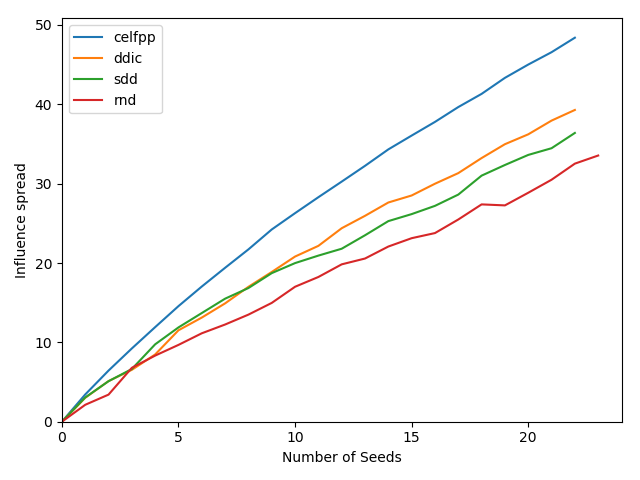
\includegraphics[scale=0.6]{img/IMG1}
\end{figure}


The second graph is still a sparse network, but with a higher activation probabilities on the edges

$nodes: 150$

$budget: 22$

$edges: np.log(n_nodes) / n_nodes$

$theta: np.random.dirichlet(np.ones(n_features), size=1)$

$features: np.random.binomial(1, 0.25, size=n_features).tolist()$

$Montecarlo iterations: 3000$

algorithm celfpp running time: 15547.94735622406

algorithm ddic running time: 406.5956394672394

algorithm sdd running time: 381.44613218307495

algorithm rnd running time: 350.65496921539307

celfpp optimal set of seeds: {35: 1, 10: 1, 132: 1, 80: 1, 81: 1, 6: 1, 68: 1, 12: 1, 102: 1, 43: 1, 19: 1, 103: 1, 51: 1, 92: 1, 50: 1, 83: 1, 139: 1, 2: 1, 97: 1, 24: 1, 123: 1, 36: 1}

ddic optimal set of seeds: {147: 1, 149: 1, 112: 1, 32: 1, 107: 1, 111: 1, 61: 1, 67: 1, 76: 1, 117: 1, 118: 1, 66: 1, 81: 1, 87: 1, 135: 1, 50: 1, 68: 1, 4: 1, 83: 1, 113: 1, 124: 1, 9: 1}

sdd optimal set of seeds: {147: 1, 149: 1, 108: 1, 112: 1, 32: 1, 107: 1, 22: 1, 82: 1, 109: 1, 111: 1, 0: 1, 56: 1, 67: 1, 117: 1, 118: 1, 76: 1, 77: 1, 90: 1, 5: 1, 47: 1, 61: 1, 87: 1}

rnd optimal set of seeds: {29: 1, 104: 1, 140: 1, 48: 1, 128: 1, 94: 1, 142: 1, 18: 1, 127: 1, 76: 1, 136: 1, 120: 1, 117: 1, 100: 1, 98: 1, 41: 1, 62: 1, 66: 1, 57: 1, 114: 1, 75: 1, 13: 1}

influence spread: [0, 54.575, 67.03966666666668, 74.19966666666669, 79.68966666666667, 83.93566666666666, 88.37266666666667, 91.723, 94.234, 96.75966666666666, 98.91499999999999, 100.95233333333334, 103.11400000000002, 104.96466666666667, 106.878, 108.68366666666668, 110.39366666666666, 112.22799999999998, 113.65899999999999, 115.04233333333332, 116.32166666666664, 117.49199999999998, 118.70399999999997]

influence spread: [0, 50.605, 56.20066666666668, 63.72766666666667, 67.04066666666664, 68.02233333333332, 68.58499999999998, 71.92899999999997, 72.92466666666665, 73.88199999999998, 73.87833333333333, 76.01066666666667, 76.35933333333334, 78.23066666666668, 78.85033333333332, 80.23033333333338, 82.63766666666668, 84.56366666666669, 85.63333333333335, 87.85966666666668, 88.29599999999998, 88.86800000000002, 89.13133333333336]

influence spread: [0, 49.774333333333324, 56.716666666666676, 57.952333333333335, 64.21933333333334, 67.71666666666667, 68.75566666666668, 69.493, 70.03599999999999, 70.59433333333332, 70.43666666666668, 70.289, 72.427, 73.74933333333331, 74.04133333333333, 76.40933333333334, 77.11233333333331, 77.49466666666666, 77.47000000000001, 78.18466666666667, 80.21233333333332, 81.43133333333334, 82.02533333333332]

influence spread: [0, 34.32433333333333, 54.349666666666664, 54.67966666666666, 57.39633333333333, 57.592666666666666, 60.356, 63.74133333333334, 66.515, 67.99866666666667, 69.90033333333334, 71.94500000000001, 72.50699999999999, 72.22233333333334, 72.47766666666666, 75.56466666666667, 77.35666666666667, 78.83466666666666, 79.496, 79.94466666666668, 80.102, 80.06766666666667, 80.13366666666667, 80.88066666666668]




\begin{figure}[H]
	\centering
	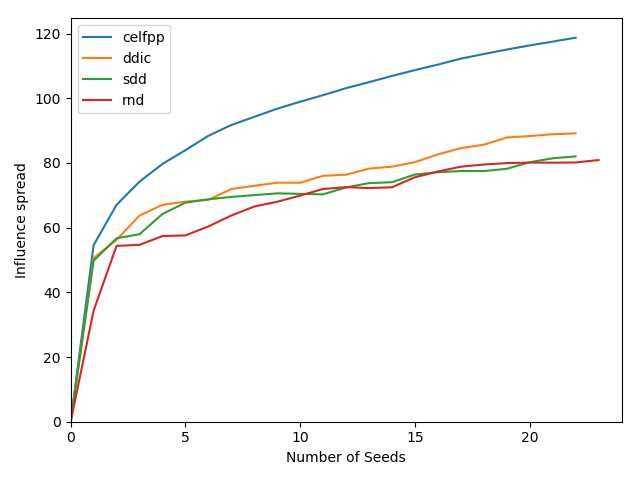
\includegraphics[scale=0.6]{img/IMG7}
\end{figure}


The third graph is still a sparse network, same as experiment 2, but with a few really strong edges

$Nodes: 150$

$Budget: 22$

$edges: np.log(n_nodes) / n_nodes$

$theta: np.random.dirichlet(np.ones(n_features), size=1)$

$features: for edge in network.edges.values():$

$if np.random.binomial(0, 0.05):$

$edge['features'] = np.random.binomial(1, 0.75, size=n_features).tolist()$

$else:$

$edge['features'] = np.random.binomial(1, 0.25, size=n_features).tolist()$

$Montecarlo iterations: 3000$

algorithm celfpp running time: 14045.999668121338

algorithm ddic running time: 402.2524745464325

algorithm sdd running time: 386.236643075943

algorithm rnd running time: 371.9336190223694

celfpp optimal set of seeds: {141: 1, 131: 1, 64: 1, 134: 1, 118: 1, 88: 1, 117: 1, 51: 1, 146: 1, 68: 1, 80: 1, 148: 1, 41: 1, 67: 1, 48: 1, 71: 1, 21: 1, 4: 1, 57: 1, 46: 1, 75: 1, 19: 1}

ddic optimal set of seeds: {55: 1, 34: 1, 62: 1, 133: 1, 139: 1, 117: 1, 31: 1, 95: 1, 107: 1, 131: 1, 12: 1, 15: 1, 70: 1, 91: 1, 144: 1, 58: 1, 59: 1, 65: 1, 67: 1, 88: 1, 149: 1, 47: 1}

sdd optimal set of seeds: {55: 1, 34: 1, 62: 1, 133: 1, 139: 1, 123: 1, 26: 1, 72: 1, 95: 1, 117: 1, 128: 1, 1: 1, 12: 1, 15: 1, 130: 1, 131: 1, 142: 1, 145: 1, 39: 1, 47: 1, 50: 1, 88: 1}

rnd optimal set of seeds: {120: 1, 64: 1, 79: 1, 103: 1, 106: 1, 32: 1, 58: 1, 61: 1, 100: 1, 128: 1, 13: 1, 88: 1, 47: 1, 25: 1, 102: 1, 60: 1, 70: 1, 77: 1, 98: 1, 51: 1, 131: 1, 122: 1}

influence spread: [0, 48.35033333333333, 60.37566666666667, 68.07766666666666, 74.58666666666664, 80.32566666666665, 84.65766666666664, 87.9303333333333, 91.01099999999995, 93.91466666666662, 96.33066666666662, 98.45499999999996, 100.75599999999997, 103.0313333333333, 104.64399999999996, 106.31499999999997, 107.85466666666663, 109.33033333333331, 111.13233333333334, 112.58066666666666, 114.10833333333332, 115.41166666666668, 116.91]

influence spread: [0, 37.32933333333335, 54.623000000000005, 56.395666666666656, 61.50766666666667, 62.44700000000002, 68.03300000000004, 69.29799999999997, 71.4906666666667, 72.94333333333329, 75.44666666666663, 77.51733333333334, 79.50966666666667, 79.83133333333338, 81.72133333333336, 83.0926666666667, 83.37266666666669, 84.36699999999996, 84.89599999999999, 87.93166666666667, 90.52899999999997, 90.89533333333334, 91.7283333333334]

influence spread: [0, 36.88266666666669, 55.249999999999986, 56.65533333333334, 61.382666666666694, 62.50800000000002, 62.69400000000002, 66.93699999999998, 67.57433333333331, 69.45866666666673, 73.4473333333333, 73.952, 73.96499999999996, 75.85433333333333, 78.318, 78.4246666666667, 79.59133333333331, 81.20533333333334, 81.78833333333331, 81.9083333333333, 82.51433333333333, 82.68333333333337, 85.68666666666671]

influence spread: [0, 10.225000000000001, 11.058666666666664, 42.949333333333335, 47.97066666666667, 47.69133333333333, 56.821, 59.489333333333335, 60.659666666666666, 65.535, 69.619, 72.01800000000003, 73.218, 77.911, 79.71166666666667, 80.326, 81.529, 81.74533333333332, 82.174, 83.339, 85.22433333333333, 88.23566666666667, 89.58500000000001, 90.733]



\begin{figure}[H]
	\centering
	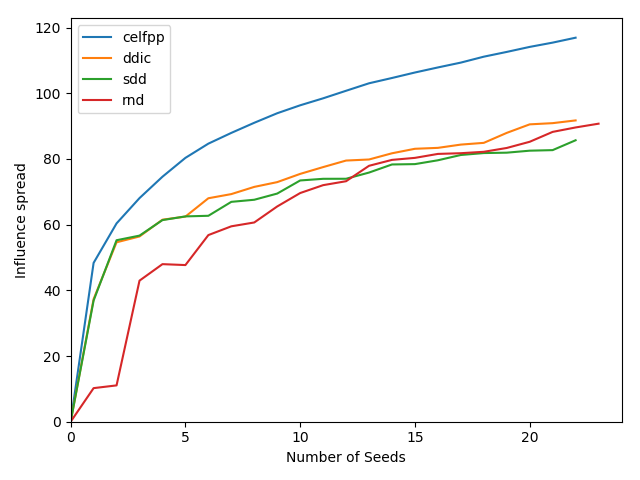
\includegraphics[scale=0.6]{img/IMG8}
\end{figure}



\subsection{Online Influence Maximization}


For this section we do not have many experimental results.
The complexity of the algorithms is too high fora common computer to run in an acceptable time (It is the same as the IM algorithms, multiplied by the number of experiments, the time horizon, the number of algorithms to run, and the complexity to run the simulation of the activation cascade).
Every run in this scenario is mediated on a number of experiments, due to the volatility of the data in the real world scenario, given by the activation cascade.


In this first example, the parameters are:

$nodes: 10$

$budget: 2$

$time horizon: 50$

$montecarlo_simulatin: 2000$

$experiment: 20$

$edges: np.log(n_nodes) / n_nodes$

$theta: np.random.dirichlet(np.ones(n_features), size=1)$

$features: for edge in network.edges.values():$

$if np.random.binomial(0, 0.05):$

$edge['features'] = np.random.binomial(1, 0.75, size=n_features).tolist()$

$else:$

$edge['features'] = np.random.binomial(1, 0.25, size=n_features).tolist()$


In the experimental results, it may seems strange that the regret is negative for the LinearUCB algorithm.
But it is not, that happened due to the few runs of the experiment that had been done, so when sampling the influence cascade from the real enviroment, it may happen that when selecting a seed of nodes, the cascade process gives an higher results than the optimal one calculated by the Influence Maximization algorithms ran on the Real network.
With more experiments and a good mediation, this problem can be eliminated.



\begin{figure}[H]
	\centering
	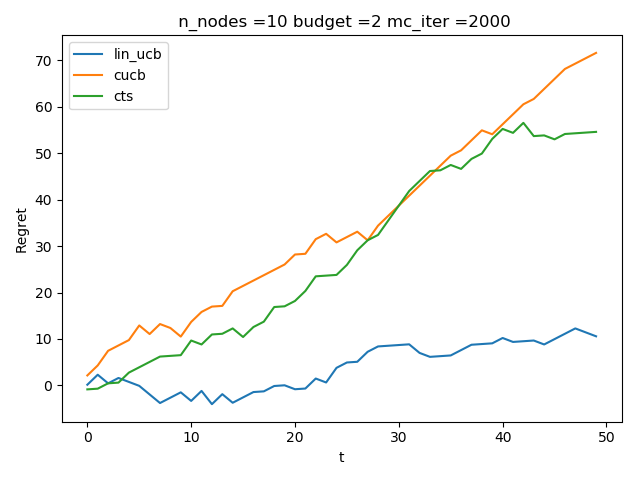
\includegraphics[scale=0.6]{img/IMG5}
\end{figure}


In the second example, the paramters are:

$nodes: 20$

$budget: 4$

$time horizon: 200$

$Montecarlo iterations: 500$( MC is 2000 in the calculation of the optimum influence spread value, 500 in the selection of the best seeds in the uncertain graph)

$experiment: 50$

$edges: np.log(n_nodes) / n_nodes$

$theta: np.random.dirichlet(np.ones(n_features), size=1)$

$features: edge['features'] = np.random.binomial(1, 0.25, size=n_features).tolist()$


Unfortunately we are not able to provide results for this example currently, as the running time of the algorithm is going to be close to 10 days on a normal computer.